\begin{frame}[t] \frametitle{LLM in contesti \emph{business}}
\framesubtitle{Riassunto delle puntate precedenti}
{\small
\onslide<1->
    \begin{minipage}[t]{\textwidth}
        \begin{itemize}[leftmargin=10pt,align=right]
            \item[\alert{\faArrowCircleRight}] Praticamente impossibile pre-addestrare un LLM (a meno che tu non sia Google, OpenAI, Mistral, Anthropic e pochissimi altri)
            \item[\alert{\faArrowCircleRight}] Utilizzare un LLM per scopi personali è un conto, adottarli in un contesto \emph{business} significa scontrarsi con problematiche di natura etica, legale ed economica
            \item[\alert{\faArrowCircleRight}] Gli LLM saranno sempre più bravi a modellare la comprensione del linguaggio$\ldots$
        \end{itemize}
        \vspace*{.5cm}
        \centering {\normalsize \textbf{\alert{\faQuestionCircleO\ $\ldots$ ma come usarli per \emph{task} specifici\\o con conoscenza che a loro manca?!}}}
    \end{minipage}
}
\end{frame}
%
\begin{frame}[t] \frametitle{\emph{Fine-tuning}}
\framesubtitle{Definizione}
{\scriptsize
\onslide<1->
    \begin{minipage}[t]{\textwidth}
        \vspace*{-.5cm}
        \begin{figure}
            \centering
            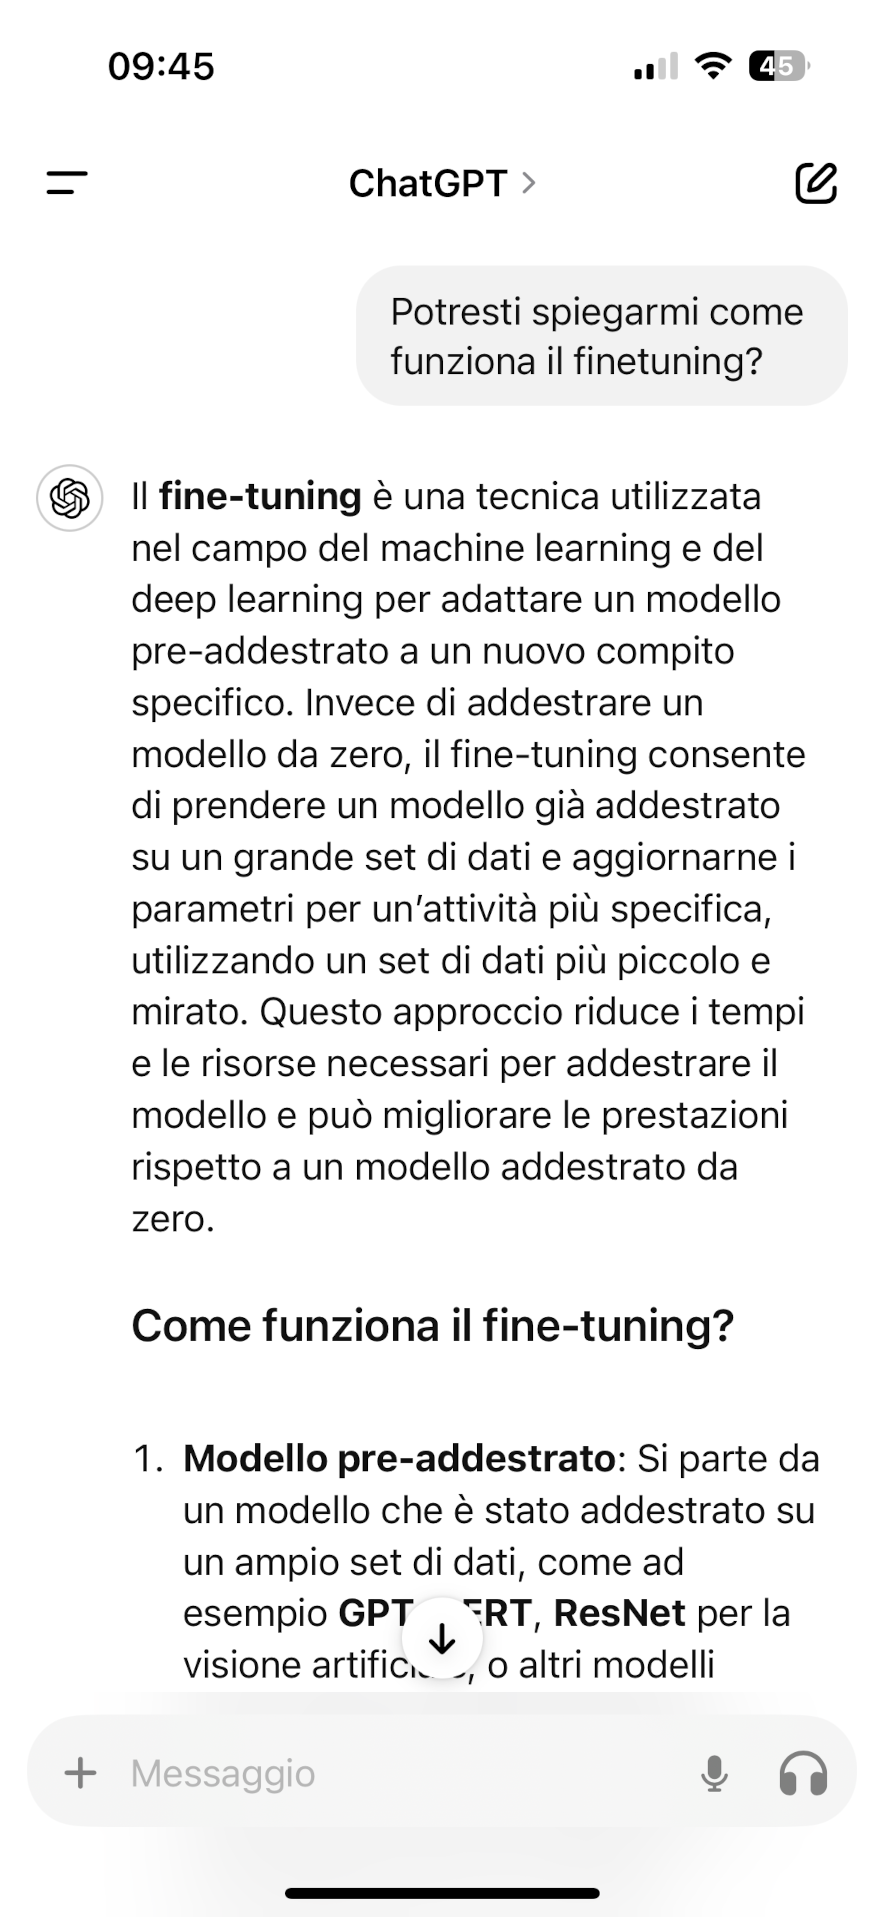
\includegraphics[width=.25\textwidth]{img/FT_1-scaled.PNG}
            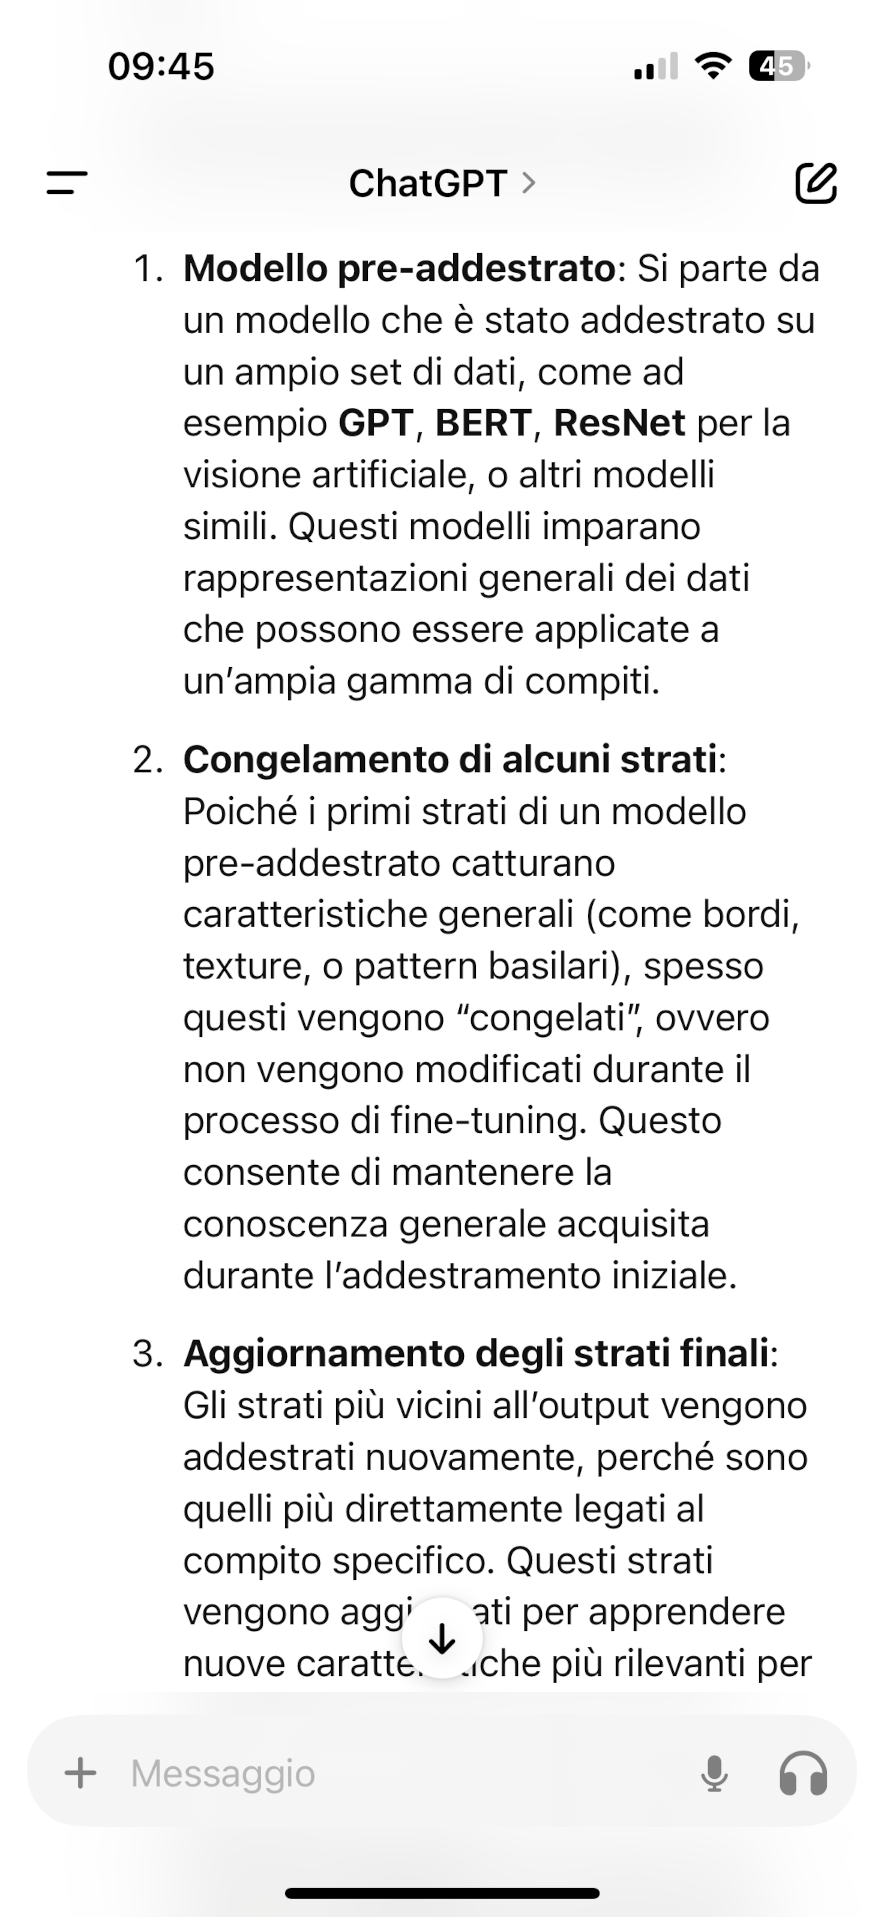
\includegraphics[width=.25\textwidth]{img/FT_2-scaled.PNG}
            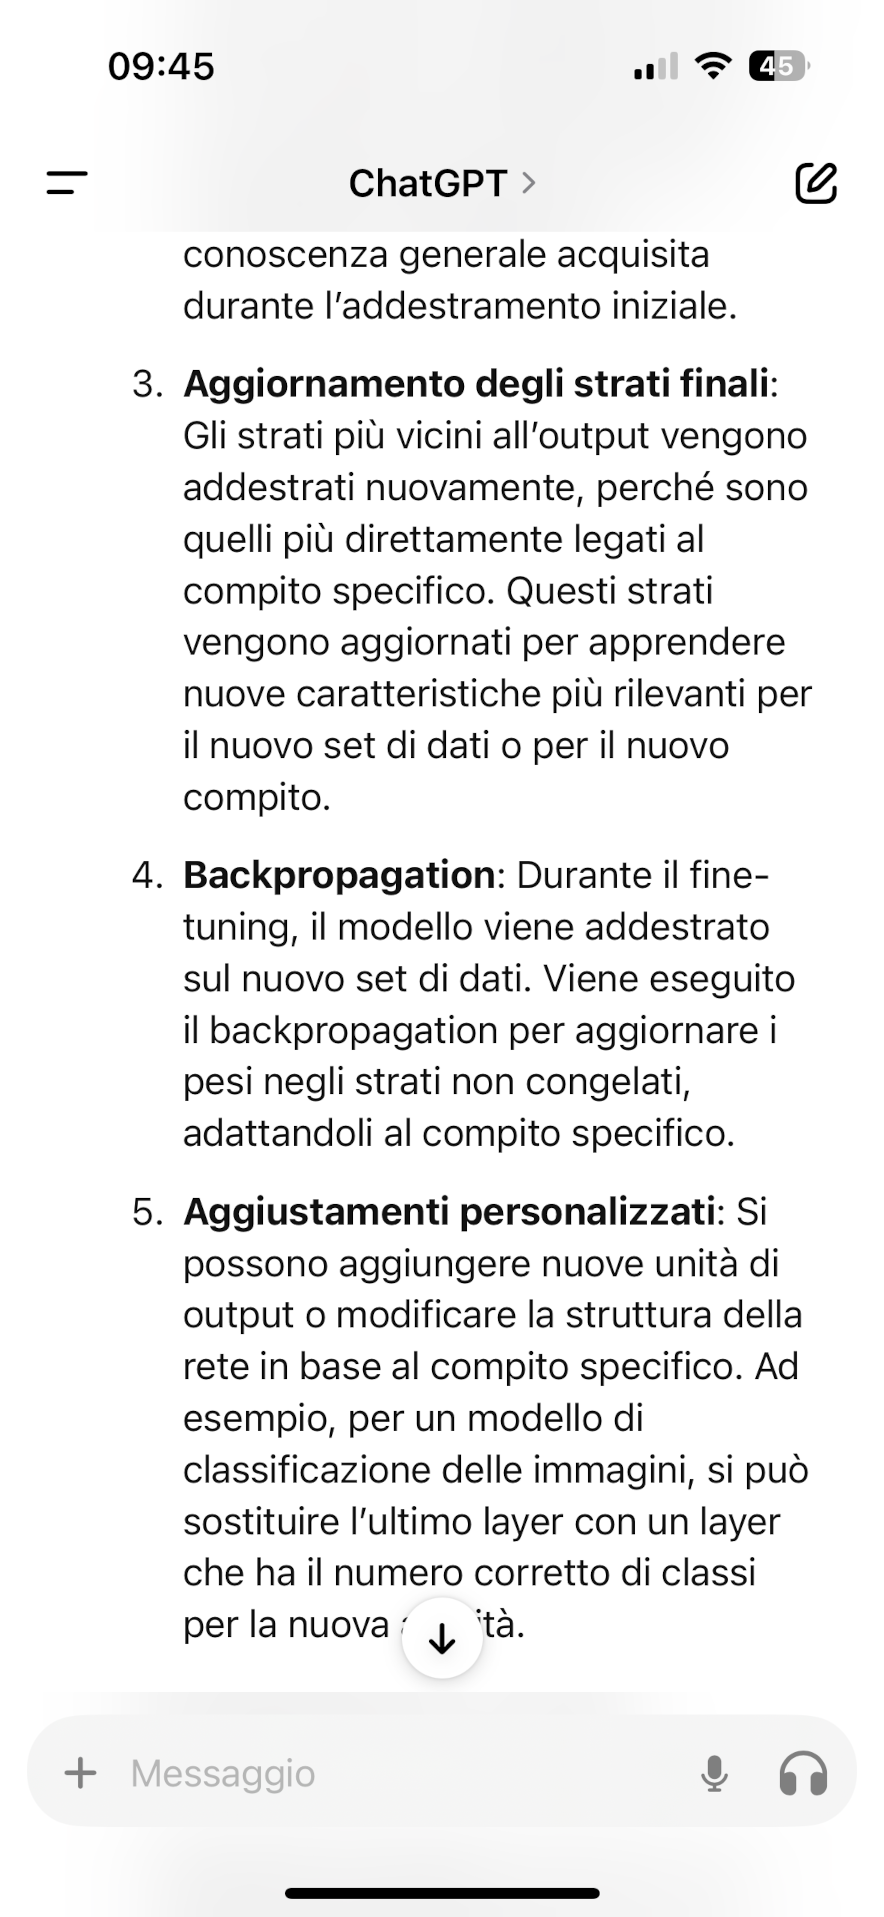
\includegraphics[width=.25\textwidth]{img/FT_3-scaled.PNG}
        \end{figure}
    \end{minipage}
}
\end{frame}
%
\begin{frame}[t] \frametitle{Addestramento neurale}
\framesubtitle{Approcci principali}
{\small
\onslide<1->
	\begin{itemize}[leftmargin=10pt,align=right]
		\item[\alert{\faArrowCircleRight}] \emph{Full learning}
		\begin{itemize}[leftmargin=10pt,align=right]
			\item[\alert{\faArrowCircleRight}] Creare una architettura neurale da zero$\ldots$
			\item[\alert{\faArrowCircleRight}] $\ldots$ oppure scegliere una architettura in letteratura (per i meno sadici)
			\item[\alert{\faArrowCircleRight}] Addestramento da zero (a partire da pesi e \emph{bias random})
		\end{itemize}
		\onslide<2->
		\item[\alert{\faArrowCircleRight}] \emph{Transfer learning}
		\begin{itemize}[leftmargin=10pt,align=right]
			\item[\alert{\faArrowCircleRight}] Sfruttare una rete neurale gi\'{a} addestrata su un altro insieme di dati di addestramento
			\item[\alert{\faArrowCircleRight}] Modificare solo alcuni strati (solitamente gli ultimi) per addestrare la rete per i propri scopi
		\end{itemize}
	\end{itemize}
	\onslide<3->
	{\footnotesize
		\begin{table}
			%% increase table row spacing, adjust to taste
			\renewcommand{\arraystretch}{1}
			\centering
			\begin{tabularx}{\textwidth}{Xp{2.5cm}p{2.5cm}}
				\toprule
				\textbf{\emph{Computer Vision}} & \textbf{\emph{Full learning}} & \textbf{\emph{Transfer learning}}\\
				\midrule

				\textbf{Numero dati addestramento} & $10^{3}$--$10^{6}$ & $10^{2}$\\
				\textbf{Computazione} & Intensiva (GPU) & Media (CPU--GPU)\\
				\textbf{Tempo di addestramento} & Giorni--settimane & Ore--giorni\\
				\textbf{Accuratezza del modello} & Alta & Variabile\\
				\bottomrule
			\end{tabularx}
		\end{table}
	}
}
\end{frame}
%
\begin{frame}[t] \frametitle{\emph{Fine-tuning}}
\framesubtitle{Il DNA del DL non mente$\ldots$}
{\small
\onslide<1->
    \begin{minipage}[t]{\textwidth}
        \begin{itemize}[leftmargin=10pt,align=right]
            \onslide<2->\item[\alert{\faArrowCircleRight}] ChatGPT parla del \emph{fine-tuning} per LLM come sinonimo di \emph{transfer learning}
            \onslide<3->\item[\alert{\faArrowCircleRight}] Si parla di \emph{\alert{full fine-tuning}} quando nessuno strato viene congelato
            \onslide<4->\item[\alert{\faArrowCircleRight}] Diverse tecniche per quanto riguarda il ``\emph{transfer tuning}''\ldots
        \end{itemize}
    \end{minipage}
}
\end{frame}
%
\begin{frame}[t] \frametitle{PEFT}
\framesubtitle{Confronto fra metodi}
{\footnotesize
\onslide<1->
    \begin{minipage}[t]{\textwidth}
        \begin{itemize}[leftmargin=10pt,align=right]
            \onslide<1->\item[\alert{\faArrowCircleRight}] \emph{\alert{P}arameter-\alert{E}fficient \alert{F}ine-\alert{T}uning}: famiglia di tecniche per ridurre i parametri da addestrare
            \begin{itemize}[leftmargin=10pt,align=right]
                \onslide<2->\item[\alert{\faArrowCircleRight}] \alert{LoRA}: decomposizione a basso rango delle matrici di peso
                \begin{itemize}[leftmargin=10pt,align=right]
                    \item[\alert{\faArrowCircleRight}] Pro: efficiente, flessibile, prestazioni eccellenti
                    \item[\alert{\faArrowCircleRight}] Contro: richiede scelta accurata di $r$ e moduli target
                \end{itemize}
                \onslide<3->\item[\alert{\faArrowCircleRight}] \alert{Adapter Layers}: inserisce piccoli \textit{layer} addestrabili tra \textit{layer} esistenti
                \begin{itemize}[leftmargin=10pt,align=right]
                    \item[\alert{\faArrowCircleRight}] Pro: modularità, facilmente componibili
                    \item[\alert{\faArrowCircleRight}] Contro: overhead di inferenza (layer aggiuntivi)
                \end{itemize}
                \onslide<4->\item[\alert{\faArrowCircleRight}] \alert{Prompt Tuning}: ottimizza solo \textit{embedding} continui del \textit{prompt}
                \begin{itemize}[leftmargin=10pt,align=right]
                    \item[\alert{\faArrowCircleRight}] Pro: estrema efficienza parametrica
                    \item[\alert{\faArrowCircleRight}] Contro: prestazioni inferiori su modelli piccoli
                \end{itemize}
            \end{itemize}
            \onslide<5->\item[\alert{\faArrowCircleRight}] LoRA attualmente considerato il miglior compromesso efficienza/prestazioni
        \end{itemize}
    \end{minipage}
}
\end{frame}
%
\begin{frame}[t] \frametitle{LoRA}
	{\scriptsize
		\onslide<1->
            \framesubtitle{Rivoluzione nel mondo dell'addestramento LLM}
            \vspace*{-.5cm}
             \begin{minipage}[t]{\textwidth}
             	\begin{figure}[ht]
                    \centering
                    \includegraphics[width=\textwidth]{img/AI-timeline-2021.png}
                \end{figure}
            \end{minipage}
            \vspace*{.3cm}
	    	\begin{minipage}[t]{.35\textwidth}
                \begin{itemize}[leftmargin=10pt,align=right]
						\onslide<2->\item[\alert{\faArrowCircleRight}] Variazione di PEFT
						\onslide<3->\item[\alert{\faArrowCircleRight}] Si riaddestrano solo un sottoinsieme $\Delta W$ di parametri esplicitamente selezionati (una sorta di \emph{transfer learning})$\ldots$
						\onslide<4->\item[\alert{\faArrowCircleRight}] $\ldots$ mantenendo fissi tutti gli altri $W$
                        \onslide<5->\item[\alert{\faArrowCircleRight}] Fissato un parametro $r$ (\alert{rango}), LoRA approssima $\Delta W$ come prodotto scalare di due matrici più piccole
                \end{itemize}
	    	\end{minipage}
    \hfill
    \onslide<1->
        \begin{minipage}[t]{.60\textwidth}
            \begin{figure}[ht]
                \centering
                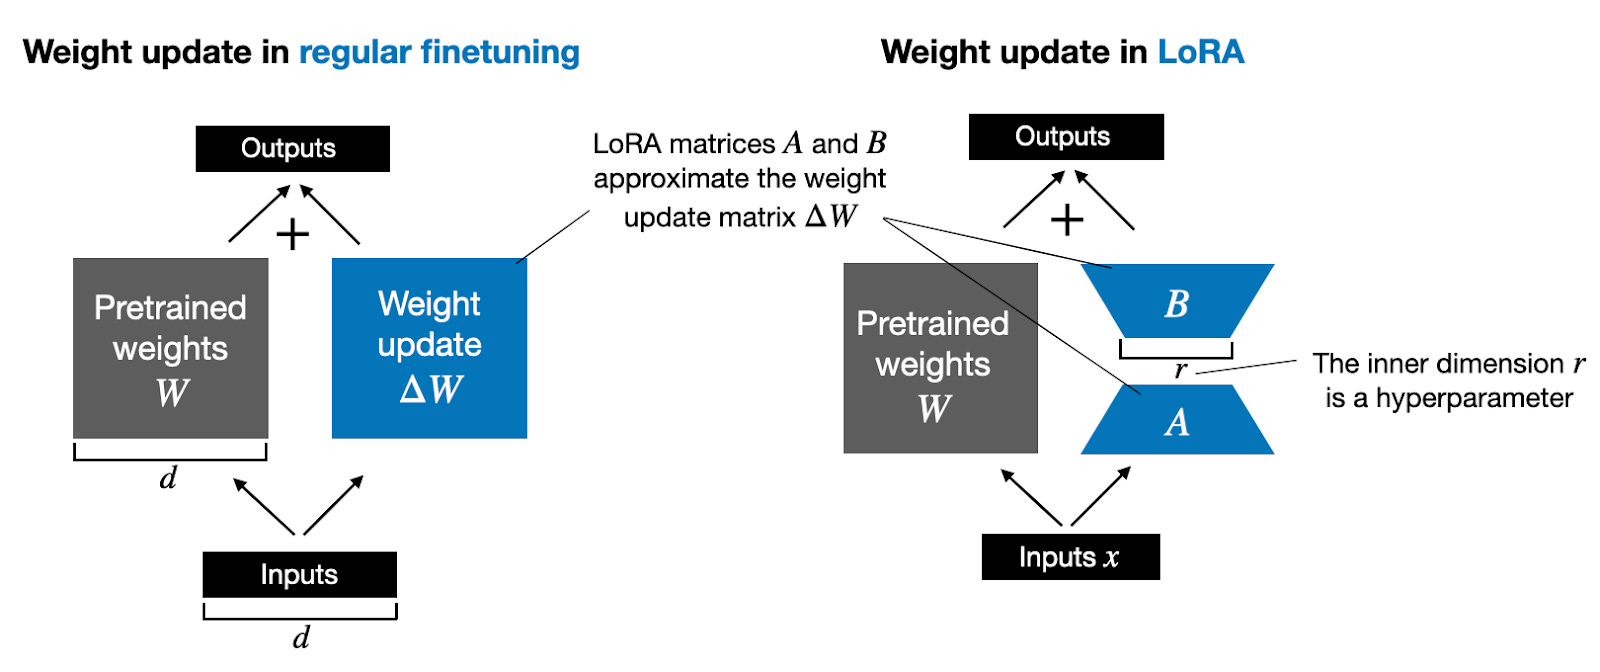
\includegraphics[width=\textwidth]{img/LoRA.png}
                {\tiny\\LoRA\\\vspace*{-1pt}\textit{\textcopyright Sebastian Raschka@Ahead of AI}}
            \end{figure}
        \end{minipage}
	}
\end{frame}
%
\begin{frame}[t] \frametitle{LoRA}
\framesubtitle{Principi algebrici}
{\tiny
    \begin{minipage}[t]{\textwidth}
        \vspace*{-.5cm}
        \begin{block}{Prodotto scalare}
            Il \emph{prodotto scalare} di matrice ($n \times r$) $A = \begin{bmatrix}
                                                                            a_{11} & a_{12} & \ldots & a_{1r}\\
                                                                            \vdots & \vdots & \vdots & \vdots\\
                                                                            a_{n1} & a_{n2} & \ldots & a_{nr}\\
            \end{bmatrix}$ e matrice ($r \times m$)
            $B = \begin{bmatrix}
                     b_{11} & b_{12} & \ldots & b_{1m}\\
                     \vdots & \vdots & \vdots & \vdots\\
                     b_{r1} & b_{r2} & \ldots & b_{rm}\\
            \end{bmatrix}$ é la matrice ($n \times m$)
            \begin{displaymath}
                A\cdot B =
                \begin{bmatrix}
                    a_{11}*b_{11} + \ldots + a_{1r}*b_{r1}& \ldots & a_{11}*b_{1m} + \ldots + a_{1r}*b_{rm}\\
                    \vdots & \vdots & \vdots\\
                    a_{n1}*b_{11} + \ldots + a_{nr}*b_{r1}& \ldots & a_{n1}*b_{1m} + \ldots + a_{nr}*b_{rm}\\
                \end{bmatrix}
            \end{displaymath}
        \end{block}
    \end{minipage}
    \begin{minipage}[t]{\textwidth}
        \vspace*{.5cm}
        {\small
        \begin{itemize}[leftmargin=10pt,align=right]
            \onslide<2->\item[\alert{\faArrowCircleRight}] In pratica, fissato $r$, LoRA computa $A$ e $B$ tale per cui $\Delta W = A\cdot B$
            \onslide<3->\item[\alert{\faArrowCircleRight}] Ma perché é così potente?!
        \end{itemize}
        }
    \end{minipage}
}
\end{frame}
%
\begin{frame}[t] \frametitle{LoRA}
\framesubtitle{Principi algebrici}
{\small
    \begin{minipage}[t]{\textwidth}
        \vspace*{-.5cm}
        \begin{block}{Esempio LoRA}
            \[
                \Delta W =
                \begin{bmatrix}
                5 & 1 & -1 & 3 & 4\\
                15 & 3 & -3 & 9 & 12\\
                35 & 7 & -7 & 21 & 28\\
                -20 & -4 & 4 & -12 & -16\\
                10 & 2 & -2 & 6 & 8\\
                \end{bmatrix} \xLongrightarrow[]{\text{LoRA($r=1$)}}
                A =
                    \begin{bmatrix}
                        1 \\
                        3 \\
                        7 \\
                        -4\\
                        2
                    \end{bmatrix},\ B=
                    \begin{bmatrix}
                        5 & 1 & -1 & 3 & 4
                    \end{bmatrix}
            \]
        \end{block}
    \end{minipage}
    \begin{minipage}[t]{\textwidth}
        \vspace*{.5cm}
        {\small
            \begin{itemize}[leftmargin=10pt,align=right]
                \onslide<2->\item[\alert{\faArrowCircleRight}] Numero parametri da salvare?
                \begin{itemize}[leftmargin=10pt,align=right]
                    \onslide<3->\item[\alert{\faArrowCircleRight}] $\Delta W$: 25
                    \item[\alert{\faArrowCircleRight}] $A$ e $B$ (totale): 10
                    \onslide<4->\item[\alert{\faArrowCircleRight}] Risparmio spazio: \alert{40\%}
                \end{itemize}
                \onslide<5->\item[\alert{\faArrowCircleRight}] La \emph{backpropagation} opera direttamente sulle rappresentazioni di $A$ e $B$!
                \onslide<6->\item[\alert{\faExclamationTriangle}] Metodo di \alert{approssimazione}, quindi a scapito della \emph{accuracy} del modello
            \end{itemize}
        }
    \end{minipage}
}
\end{frame}
%
\begin{frame}[t] \frametitle{LoRA vs \emph{Full Fine-tuning}}
\framesubtitle{Confronto pratico}
{\scriptsize
\onslide<1->
    \begin{minipage}[t]{\textwidth}
        {\scriptsize
            \begin{table}
                \renewcommand{\arraystretch}{1.3}
                \centering
                \begin{tabularx}{\textwidth}{Xp{3.5cm}p{3.5cm}}
                    \toprule
                    \textbf{Aspetto} & \textbf{\emph{Full Fine-tuning}} & \textbf{LoRA}\\
                    \midrule
                    \textbf{Parametri addestrabili} & Tutti ($\sim$100\%) & 0.1--1\% del totale\\
                    \textbf{Memoria GPU richiesta} & Molto alta (es. 80GB per 7B) & Ridotta (es. 16GB per 7B)\\
                    \textbf{Tempo addestramento} & Lungo & Significativamente ridotto\\
                    \textbf{Accuratezza finale} & Massima & Comparabile (95-99\%)\\
                    \textbf{Rischio \textit{overfitting}} & Alto con pochi dati & Basso\\
                    \textbf{\textit{Storage} adattatori} & Modello completo (GBs) & Solo adattatori (MBs)\\
                    \textbf{\textit{Multi-task}} & Richiede modelli separati & Adattatori intercambiabili\\
                    \bottomrule
                \end{tabularx}
            \end{table}
        }
    \end{minipage}
}
\end{frame}
%
\begin{frame}[t] \frametitle{\emph{Quantization}}
\framesubtitle{Ottimizzazione per \emph{full fine-tuning}}
{\scriptsize
\onslide<1->
    \begin{minipage}[t]{\textwidth}
        \vspace*{-.5cm}
        \begin{itemize}[leftmargin=10pt,align=right]
            \onslide<1->\item[\alert{\faArrowCircleRight}] Decidere la precisione dei parametri del modello (ovvero, \emph{quantizzandolo})
        \end{itemize}
    \end{minipage}
    \begin{minipage}[t]{\textwidth}
        \vspace*{.2cm}
            \begin{figure}
                \centering
                \includegraphics[width=.7\textwidth]{img/quantization-no-bg.png}
                {\tiny\\Quantizzazione\\\vspace*{-1pt}\textit{\textcopyright Cerebras}}
            \end{figure}
    \end{minipage}
    \begin{minipage}[t]{\textwidth}
        \vspace*{.2cm}
        \begin{itemize}[leftmargin=10pt,align=right]
            \onslide<2->\item[\alert{\faArrowCircleRight}] Quantizzazione a \texttt{float16} e \texttt{bfloat16} usati maggiormente per addestramento
            \item[\alert{\faArrowCircleRight}] \texttt{bfloat16} generalmente preferito a \texttt{float16}
            \onslide<3->\item[\alert{\faArrowCircleRight}] Addestramento a \texttt{float32} riservato alle \emph{big companies}
            \onslide<4->\item[\alert{\faArrowCircleRight}] Quantizzazioni inferiori disponibili (\texttt{int8}, \texttt{int4}), ma consigliate per inferenza
        \end{itemize}
    \end{minipage}
}
\end{frame}
%
\begin{frame}[t] \frametitle{\emph{Quantization}}
\framesubtitle{Visione concettuale}
{\footnotesize
\onslide<1->
    \begin{minipage}[t]{\textwidth}
        \vspace*{-.3cm}
        \begin{figure}
            \centering
            \includegraphics[width=.8\textwidth]{img/quantization_concept_no_bg.png}
            {\tiny\\Quantizzazione\\\vspace*{-1pt}\textit{\textcopyright jeremy jouvance@GoPenAI}}
        \end{figure}
    \end{minipage}
    \begin{minipage}[t]{\textwidth}
            \vspace*{.3cm}
        \begin{itemize}[leftmargin=10pt,align=right]
            \onslide<2->\item[\alert{\faArrowCircleRight}] A favore del peso del modello in memoria e ai tempi di addestramento$\ldots$
            \onslide<3->\item[\alert{\faArrowCircleRight}] $\ldots$ a scapito dell'accuratezza in fase di inferenza
        \end{itemize}
    \end{minipage}
}
\end{frame}
%
\begin{frame}[t] \frametitle{\emph{Quantization}}
\framesubtitle{Strategie e formati avanzati}
{\footnotesize
\onslide<1->
    \begin{minipage}[t]{\textwidth}
        \begin{itemize}[leftmargin=10pt,align=right]
            \onslide<1->\item[\alert{\faArrowCircleRight}] Quantizzazione terminato il processo di addestramento (\alert{P}ost \alert{T}raining \alert{Q}uantization -- PTQ)
            \begin{itemize}[leftmargin=10pt,align=right]
                \onslide<2->\item[\alert{\faArrowCircleRight}] \alert{GPTQ}: quantizzazione post-addestramento per GPU, ottimizzata per inferenza veloce
                \onslide<3->\item[\alert{\faArrowCircleRight}] \alert{GGUF/GGML}: formato quantizzato per CPU e Metal (Apple Silicon), popolare per uso locale
            \end{itemize}
            \onslide<4->\item[\alert{\faArrowCircleRight}] Quantizzazione durante l'addestramento (\emph{\alert{Q}uantization-\alert{A}ware \alert{T}raining -- QAT})
            \begin{itemize}[leftmargin=10pt,align=right]
                \onslide<5->\item[\alert{\faArrowCircleRight}] \alert{BitsAndBytes (\texttt{bitsandbytes})}: libreria per quantizzazione dinamica 8-bit e 4-bit
            \end{itemize}
        \end{itemize}
    \end{minipage}
    \onslide<6->
    \begin{minipage}[t]{\textwidth}
        \vspace*{.7cm}
        {\scriptsize
            \begin{table}
                \renewcommand{\arraystretch}{1.2}
                \centering
                \begin{tabularx}{\textwidth}{Xp{2.5cm}p{3cm}p{2cm}}
                    \toprule
                    \textbf{Formato} & \textbf{Riduzione memoria} & \textbf{Uso principale} & \textbf{Accuratezza}\\
                    \midrule
                    \texttt{int8} & $\sim$50\% & Inferenza & Alta\\
                    \texttt{int4} & $\sim$75\% & Inferenza & Media-Alta\\
                    \texttt{GPTQ} & $\sim$75\% & Inferenza (GPU) & Alta\\
                    \texttt{GGUF} & 50-80\% & Inferenza (CPU) & Variabile\\
                    \bottomrule
                \end{tabularx}
            \end{table}
        }
    \end{minipage}
}
\end{frame}
%
\begin{frame}[t] \frametitle{QLoRA}
{\small
\onslide<1->
\framesubtitle{Cosa sarà mai$\ldots$?}
\vspace*{-.5cm}
    \begin{minipage}[t]{\textwidth}
        \begin{figure}[ht]
            \centering
            \includegraphics[width=\textwidth]{img/AI-timeline-2023.png}
        \end{figure}
    \end{minipage}
    \vspace*{.3cm}
    \begin{minipage}[t]{\textwidth}
        \begin{itemize}[leftmargin=10pt,align=right]
            \onslide<2->\item[\alert{\faArrowCircleRight}] Decomposizione LoRA + \emph{Quantization}$\ldots$
            \onslide<3->\item[\alert{\faArrowCircleRight}] $\ldots$ tutto qui.
        \end{itemize}
    \end{minipage}
}
\end{frame}
%
\begin{frame}[t] \frametitle{QLoRA}
\framesubtitle{Dettagli tecnici}
{\small
\onslide<1->
    \begin{minipage}[t]{\textwidth}
        \begin{itemize}[leftmargin=10pt,align=right]
            \onslide<1->\item[\alert{\faArrowCircleRight}] QLoRA introduce ottimizzazioni chiave per ridurre drasticamente l'uso di memoria
            \begin{itemize}[leftmargin=10pt,align=right]
                \onslide<2->\item[\alert{\faArrowCircleRight}] Congelamento e quantizzazione totale del modello originale a 4 bit
                \begin{itemize}[leftmargin=10pt,align=right]
                    \item[\alert{\faArrowCircleRight}] \alert{4-bit NormalFloat (NF4)}: quantizzazione ottimizzata per distribuzioni normali dei pesi
                \end{itemize}
                \onslide<3->\item[\alert{\faArrowCircleRight}] \alert{Paged Optimizers}: gestione della memoria simile alla memoria virtuale del SO
            \end{itemize}
            \onslide<4->\item[\alert{\faArrowCircleRight}] Solo gli adattatori LoRA vengono addestrati in precisione maggiore (tipicamente \texttt{bfloat16})
            \onslide<5->\item[\alert{\faExclamationTriangle}] Riduzione tempi di addestramento e spazio richiesto rispetto a LoRA
            \begin{itemize}[leftmargin=10pt,align=right]
                \item[\alert{\faArrowCircleRight}] \emph{Fine-tuning} di modelli da 65B parametri su GPU \textit{consumer} (24GB)
            \end{itemize}            
        \end{itemize}
    \end{minipage}
}
\end{frame}
%
\begin{frame}[t] \frametitle{\emph{Fine-tuning}}
\framesubtitle{Requisiti hardware e calcoli di memoria}
\vspace*{-.7cm}
{\scriptsize
\onslide<1->
    \begin{minipage}[t]{\textwidth}
        \begin{itemize}[leftmargin=10pt,align=right]
            \onslide<1->\item[\alert{\faExclamationTriangle}] Stima memoria GPU necessaria per \emph{fine-tuning}?!
            \begin{itemize}[leftmargin=10pt,align=right]
                \onslide<2->\item[\alert{\faArrowCircleRight}] \alert{\emph{Full fine-tuning}}: $\text{Memoria} \approx 4 \times \text{parametri} \times \text{bytes per parametro}$
                \begin{itemize}[leftmargin=10pt,align=right]
                    \item[\alert{\faExclamationTriangle}] Fattore $4\times$: modello + gradienti + stati ottimizzatore
                \end{itemize}
                \onslide<3->\item[\alert{\faArrowCircleRight}] \alert{LoRA}: $\text{Memoria} \approx 2\times \text{n}_{\text{params}} + \text{n}_{\text{LoRA\_adapters}} \times \text{dim}_{\text{LoRA\_adapters}}$, $\text{dim}_{\text{LoRA\_adapters}} \approx 200MB$
                \onslide<4->\item[\alert{\faArrowCircleRight}] \alert{QLoRA}: $\text{Memoria} \approx .5\times \text{n}_{\text{params}} + \text{n}_{\text{LoRA\_adapters}} \times \text{dim}_{\text{LoRA\_adapters}}$, $\text{dim}_{\text{LoRA\_adapters}} \approx 200MB$
            \end{itemize}
            \onslide<5->\item[\alert{\faArrowCircleRight}] \emph{Batch size} e lunghezza sequenza impattano significativamente
            \onslide<6->\item[\alert{\faExclamationTriangle}] Considerare anche memoria per attivazioni intermedie ($\approx 50\%$ aggiuntivo)
        \end{itemize}
    \end{minipage}
    \onslide<7->
    \begin{minipage}[t]{\textwidth}
        \vspace*{.3cm}
        \begin{figure}[ht]
            \centering
            \includegraphics[width=.7\textwidth]{img/gpu-llm-calculator.png}
            {\tiny\\\alert{\faLink}\ \url{https://apxml.com/tools/vram-calculator}}
        \end{figure}
    \end{minipage}
}
\end{frame}
%
\begin{frame}[t] \frametitle{\emph{Fine-tuning}}
\framesubtitle{\emph{Best practices}}
{\small
\onslide<1->
    \begin{minipage}[t]{\textwidth}
        \begin{itemize}[leftmargin=10pt,align=right]
            \onslide<1->\item[\alert{\faArrowCircleRight}] Preparazione \textit{dataset}
            \begin{itemize}[leftmargin=10pt,align=right]
                \onslide<2->\item[\alert{\faArrowCircleRight}] Qualità $>$ Quantità: meglio 1000 esempi di alta qualità che 10000 rumorosi
                \onslide<3->\item[\alert{\faArrowCircleRight}] Formattazione consistente: usare \textit{template} uniformi per prompt e risposte
                \onslide<4->\item[\alert{\faArrowCircleRight}] Bilanciamento: evitare sbilanciamenti tra categorie o lunghezze
            \end{itemize}
            \onslide<5->\item[\alert{\faArrowCircleRight}] Iperparametri addestramento
            \begin{itemize}[leftmargin=10pt,align=right]
                \onslide<6->\item[\alert{\faArrowCircleRight}] \emph{Learning rate}: tipicamente $[5\text{e-}5, 1\text{e-}4]$ per \emph{full}, $[$3\text{e-}4, 1\text{e-}3$]$ per LoRA
                \onslide<7->\item[\alert{\faArrowCircleRight}] Poche epoche: 1-5 epoche solitamente sufficienti (rischio \emph{overfitting})
            \end{itemize}
            \onslide<8->\item[\alert{\faArrowCircleRight}] Prevenzione \emph{overfitting}
            \begin{itemize}[leftmargin=10pt,align=right]
                \onslide<9->\item[\alert{\faArrowCircleRight}] \emph{Early stopping}: monitorare \textit{loss} su \textit{validation set}
                \onslide<10->\item[\alert{\faArrowCircleRight}] \textit {Dropout} e \emph{weight decay} per regolarizzazione
                \onslide<11->\item[\alert{\faArrowCircleRight}] \textit{Validation} regolare su esempi reali del dominio textit{target}
            \end{itemize}
        \end{itemize}
    \end{minipage}
}
\end{frame}
%
\begin{frame}[t] \frametitle{\emph{Fine-tuning}}
\framesubtitle{Quando utilizzare cosa}
{\small
\onslide<1->
    \begin{minipage}[t]{\textwidth}
        \begin{itemize}[leftmargin=10pt,align=right]
            \onslide<1->\item[\alert{\faArrowCircleRight}] \emph{Full fine-tuning}
            \begin{itemize}[leftmargin=10pt,align=right]
                \onslide<2->\item[\alert{\faArrowCircleRight}] Cambio drastico di dominio (es. da generale a medico/legale)
                \onslide<3->\item[\alert{\faArrowCircleRight}] \textit{Dataset} molto grandi ($>$100K esempi di alta qualità)
                \onslide<4->\item[\alert{\faArrowCircleRight}] Risorse computazionali abbondanti
                \onslide<5->\item[\alert{\faArrowCircleRight}] Massima accuratezza richiesta per il \emph{task}
            \end{itemize}
            \onslide<1->\item[\alert{\faArrowCircleRight}] LoRA/QLoRA
            \begin{itemize}[leftmargin=10pt,align=right]
                \onslide<6->\item[\alert{\faArrowCircleRight}] Adattamento stile, tono, formato \textit{output}
                \onslide<7->\item[\alert{\faArrowCircleRight}] Comportamenti specifici o \emph{task} strutturati
                \onslide<8->\item[\alert{\faArrowCircleRight}] \textit{Dataset} 1K--100K esempi, risorse \textit{hardware} limitate
                \onslide<9->\item[\alert{\faArrowCircleRight}] Necessità di gestire multipli adattatori per \emph{task} diversi
            \end{itemize}
        \end{itemize}
    \end{minipage}
}
\end{frame}
%